\documentclass[12pt]{exam}
\usepackage{xparse}
\usepackage{rosoff-vector-macros}
\usepackage{rosoff}
\usepackage{graphicx}
\DeclareGraphicsExtensions{.jpg, .png}
\usepackage{fourier}
\usepackage{MnSymbol}
\usepackage{amsthm}
\usepackage{paralist,enumerate,listings}
\usepackage{siunitx}
\frenchspacing
\usepackage{parskip}
\usepackage{hyperref}
\firstpageheader{}{}{}
\runningheader{\textbf{Fall 2013}}
 {}
 {\textbf{Math 251}}
 %{\emph{Page \thepage~of \numpages}}
\runningheadrule

\pagestyle{head}

\begin{document}
\noindent
\textbf{{\large Math 251 \hfill Quiz 03 (WeBWorK 4)}}
% \hfill Name: \underline{\hspace{0.5in}Answers\hspace{2in}}

\noindent
October 4, 2013; 10 minutes \hfill Name: \underline{\hspace{3in}} 

\noindent

\noindent
This quiz is \emph{open-note}, but no books or calculators may be used.
In calculation, you can show work at your discretion, but remember that
I can't give partial credit for calculations I can't see. Explain
anything that seems to need explaining.

\begin{questions} 

\question A contour map for a function $f(x,y)$ is pictured below. Select the best answer to each of the questions regarding the partial derivatives $f_x$ and $f_y$ at the various labeled points.
\begin{figure}[ht]
    \begin{minipage}[b]{0.45\linewidth}
        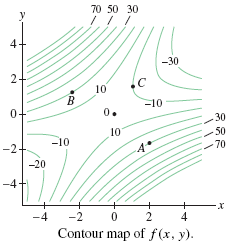
\includegraphics[width=\textwidth]{images/contour.png}
    \end{minipage} \hspace*{1cm}
    \begin{minipage}[b]{0.45\linewidth}
        \begin{parts}
        \part At point $A$:
        \begin{checkboxes}
            \choice $f_x > 0$ and $f_y > 0$
            \choice $f_x < 0$ and $f_y > 0$
            \choice $f_x > 0$ and $f_y < 0$
            \choice $f_x < 0$ and $f_y < 0$
        \end{checkboxes}
        \part At point $B$:
        \begin{checkboxes}
            \choice $f_x > 0$ and $f_y > 0$
            \choice $f_x < 0$ and $f_y > 0$
            \choice $f_x > 0$ and $f_y < 0$
            \choice $f_x < 0$ and $f_y < 0$
        \end{checkboxes}
        \part At point $C$:
        \begin{checkboxes}
            \choice $f_x > 0$ and $f_y > 0$
            \choice $f_x < 0$ and $f_y > 0$
            \choice $f_x > 0$ and $f_y < 0$
            \choice $f_x < 0$ and $f_y < 0$
        \end{checkboxes}
        \end{parts}
    \end{minipage}
\end{figure}

Note: the graph of the function $f(x,y)$ is called a "saddle surface". Can you see why?

\dwrspace{1}

\question Compute $g_x$ and $g_y$ if $g$ is given by the formula 
\begin{equation*}
    g(x,y) = \frac{4x}{(x^2 + y^2)^{3/2}}.    
\end{equation*}
Do not simplify your answers.

\dwrspace{6}

\end{questions} 

\end{document}